\documentclass[11pt]{article} 
\setlength{\oddsidemargin}{0.0in}
\setlength{\evensidemargin}{0.0in}
\setlength{\topmargin}{-0.25in}
\setlength{\headheight}{0in}
\setlength{\headsep}{0in}
\setlength{\textwidth}{6.5in}
\setlength{\textheight}{9.25in}
\setlength{\parindent}{0in}
\setlength{\parskip}{2mm}
\newcommand\tab[1][0.5cm]{\hspace*{#1}}
\usepackage{listings}
\usepackage{amsmath,amsfonts,amsthm, amssymb} % Math packages
\usepackage[utf8]{inputenc}
\usepackage{graphicx}
\usepackage{subcaption}
\usepackage{comment}

\title{ECS 189G Homework 2}
\author{Bochao Xin, Dianfeng Jiang, Melissa Goh, Shikun Huang}
\date{Due: 24 February 2020 (Monday)}

\begin{document}

\maketitle

\section{Problem A}
Our intuition to predicting ratings is based on factors that fundamentally represent the user's
personality. Some features we considered are age, usernum, and occupation. To elaborate on this,
we think that including usernum as a feature would let us know their rating based on how harshly
or leniently a user rates their movies, based on their user ID. 

\begin{figure}[ht!]
\begin{center}
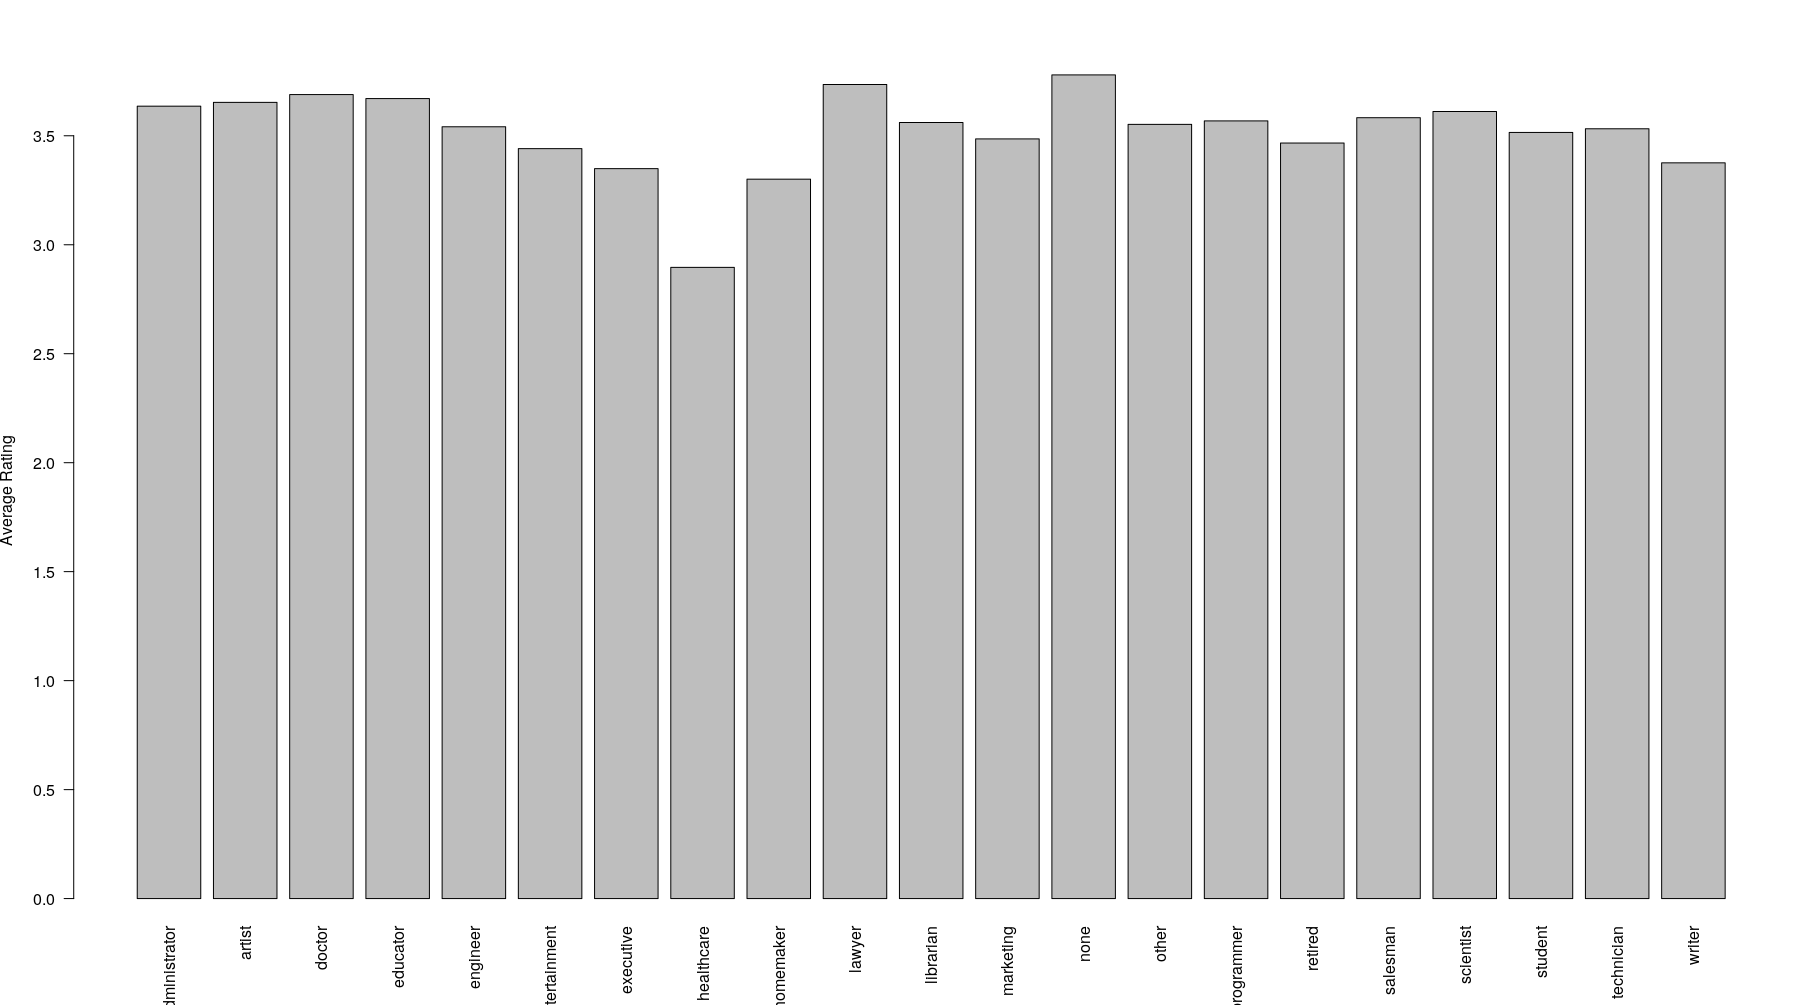
\includegraphics[width=0.8\textwidth]{ratingxocc.png}
\caption{Average Rating vs. Occupation}
\end{center}
\end{figure}

Intuitively, occupation reflects a person's personality. We plotted the average rating given by
each occupation. As shown in the plot, the ratings are not very uniform, which would probably
make Occupation a good feature to predict ratings. Since age likely affects
the kind of occupation a person has, we decided to use the interaction term `age` and `occ` to predicting
ratings. The MAPE obtained from this set of features is 0.8752.

\begin{verbatim}
    > lmout <- lm(rating ~ age*occ, data=trnSet)
    summary(lmout)
    > summary(lmout)
    
    Call:
    lm(formula = rating ~ age * occ, data = trnSet)
    
    Residuals:
        Min      1Q  Median      3Q     Max 
    -3.5559 -0.5763  0.3376  0.5374  2.8331 
    
    Coefficients:
                           Estimate Std. Error t value Pr(>|t|)    
    (Intercept)           3.3457294  0.0523707  63.885  < 2e-16 ***
    age                   0.0073463  0.0012955   5.670 1.43e-08 ***
    occartist            -0.6775732  0.1078113  -6.285 3.30e-10 ***
    occdoctor            -0.1125594  0.1831937  -0.614 0.538934    
    occeducator           0.3647334  0.0734661   4.965 6.89e-07 ***
    occengineer          -0.0359133  0.0688078  -0.522 0.601716    
    occentertainment      0.6526975  0.1318031   4.952 7.36e-07 ***
    occexecutive         -1.3817756  0.0913665 -15.123  < 2e-16 ***
    occhealthcare        -2.1325458  0.0901122 -23.665  < 2e-16 ***
    occhomemaker         -0.3012994  0.2346490  -1.284 0.199130    
    occlawyer             0.0806203  0.1262801   0.638 0.523199    
    occlibrarian          0.0534024  0.0785553   0.680 0.496629    
    occmarketing          0.3054019  0.1264570   2.415 0.015734 *  
    occnone               0.5380508  0.1263167   4.260 2.05e-05 ***
    occother              0.1970186  0.0646248   3.049 0.002299 ** 
    occprogrammer        -0.0590576  0.0695120  -0.850 0.395548    
    occretired           -0.3376369  0.4328787  -0.780 0.435404    
    occsalesman           0.1159735  0.1359053   0.853 0.393473    
    occscientist         -0.0424774  0.1416788  -0.300 0.764319    
    occstudent            0.2005008  0.0630880   3.178 0.001483 ** 
    occtechnician         0.2030625  0.0863610   2.351 0.018709 *  
    occwriter            -0.8011493  0.0768054 -10.431  < 2e-16 ***
    age:occartist         0.0247203  0.0032503   7.606 2.86e-14 ***
    age:occdoctor         0.0056768  0.0049181   1.154 0.248394    
    age:occeducator      -0.0083699  0.0017469  -4.791 1.66e-06 ***
    age:occengineer      -0.0007054  0.0017976  -0.392 0.694775    
    age:occentertainment -0.0267839  0.0043092  -6.216 5.14e-10 ***
    age:occexecutive      0.0302180  0.0023624  12.791  < 2e-16 ***
    age:occhealthcare     0.0360066  0.0022189  16.227  < 2e-16 ***
    age:occhomemaker      0.0009872  0.0068782   0.144 0.885874    
    age:occlawyer         0.0013949  0.0034506   0.404 0.686035    
    age:occlibrarian     -0.0031238  0.0019904  -1.569 0.116554    
    age:occmarketing     -0.0116446  0.0033326  -3.494 0.000476 ***
    age:occnone          -0.0114218  0.0045476  -2.512 0.012021 *  
    age:occother         -0.0071173  0.0017077  -4.168 3.08e-05 ***
    age:occprogrammer     0.0014500  0.0018701   0.775 0.438121    
    age:occretired        0.0001103  0.0070637   0.016 0.987546    
    age:occsalesman      -0.0038728  0.0037978  -1.020 0.307855    
    age:occscientist      0.0012039  0.0038758   0.311 0.756089    
    age:occstudent       -0.0085517  0.0020196  -4.234 2.29e-05 ***
    age:occtechnician    -0.0079412  0.0024493  -3.242 0.001186 ** 
    age:occwriter         0.0168032  0.0020383   8.244  < 2e-16 ***
    ---
    Signif. codes:  0 ‘***’ 0.001 ‘**’ 0.01 ‘*’ 0.05 ‘.’ 0.1 ‘ ’ 1
    
    Residual standard error: 1.109 on 94958 degrees of freedom
    Multiple R-squared:  0.02956,   Adjusted R-squared:  0.02914 
    F-statistic: 70.54 on 41 and 94958 DF,  p-value: < 2.2e-16
\end{verbatim}
\section{Problem B}

\end{document}